\documentclass[11pt]{report}

\usepackage[utf8]{inputenc}
\usepackage{times}

\usepackage{url}

\usepackage{amsmath, amstext}
\usepackage{array}

\usepackage{enumerate}

\usepackage{pstricks, pst-node, pst-tree}

\usepackage{graphicx}

\usepackage{auto-pst-pdf}

%\usepackage{draftcopy}

%%%%%%%%%%%%%
% Softwares %
%%%%%%%%%%%%%
\def\amlet{\textsf{AMLET}}
\def\ophelia{\textsf{OPHELIA}}
\def\oratio{\textsf{ORATIO}}
\def\atlas{\textsf{ATLAS}}
\def\blas{\textsf{BLAS}}
\def\cblas{\textsf{CBLAS}}

\def\cygwin{\textsf{Cygwin}}
\def\gauss{\textsf{GAUSS}}
\def\gcc{\textsf{gcc}}
\def\gfortran{\textsf{gfortran}}
\def\gsl{\textsf{GSL}}
\def\limdep{\textsf{LIMDEP}}
\def\mingw{\textsf{MinGW}}
\def\software#1{\textsf{#1}}

\def\amletarch{amlet-0.10.0.tar.gz}
\def\atlasarch{atlas3.6.0.tar.bz2}
\def\ctoolsarch{ctools-0.5.4.tar.gz}
\def\dclarch{dcl-0.1.0.tar.gz}
\def\dstructarch{dstruct-0.5.3.tar.gz}
\def\expatarch{expat-2.0.0.tar.gz}
\def\mocaarch{moca-0.1.1.tar.gz}
\def\nlparch{nlp-0.5.0.tar.gz}
\def\ntoolsarch{ntools-0.6.0.tar.gz}
\def\statarch{stat-0.5.0.tar.gz}

\def\mail{\url{bastin@iro.umontreal.ca}}

%%%%%%%%%
% Title %
%%%%%%%%%
\author{Fabian Bastin\\\mail}
\title{\amlet{} User's Guide}
\date{\today}

\def\version{0.13.1}

\usepackage{doc}
\usepackage{makeidx}
\newcommand{\Index}[1]{#1\index{#1}}
\makeindex

\begin{document}

\begin{titlepage}
{\Huge {\bf AMLET}} 

{\huge Reference manual}

\vspace*{\stretch{1}}

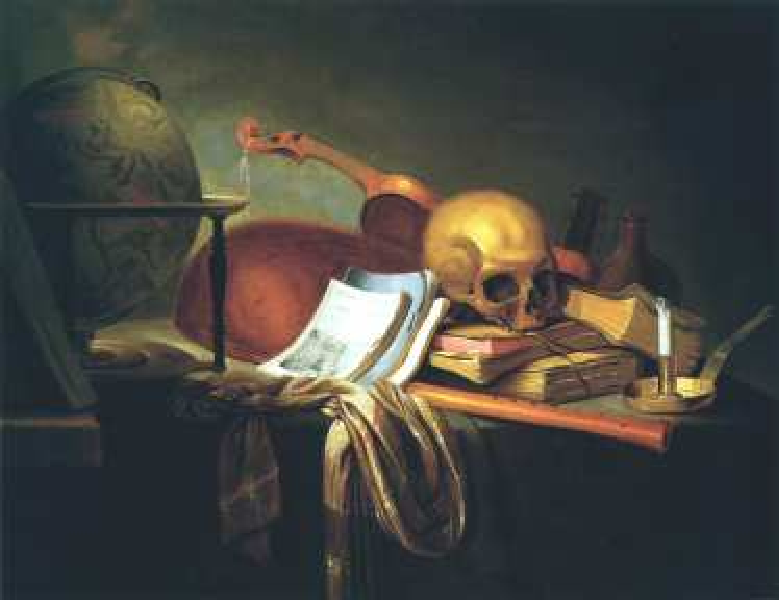
\includegraphics{pst.pdf}

\vspace*{\stretch{1}}

Fabian Bastin\hspace*{\stretch{1}}{\large  \today}

\date{}

\end{titlepage}

\begin{abstract}
This document explains how to install and use the software
\amlet{} v\version, designed to estimate multinomial and mixed
logit models.
The current documentation is unfortunately far from be completed,
and is full omissions and possibly errors.
Any suggestion concerning this document
and/or the software should be send to \mail.

The latest version of this document, as well as the software itself,
can be retrieved at the internet address \url{http://amlet.slashbin.net}.
\end{abstract}

\tableofcontents

\chapter{Introduction}

\section{What is \amlet?}

\amlet{} is an acronym for \underline{A}nother \underline{M}ixed
\underline{L}ogit \underline{E}stimation \underline{T}ool.
As its name suggests, it is a software mainly designed to estimate various
kind of mixed logit models.
It can be used either as a standalone program, either as a C library.
\amlet{} is an open source project (see Appendix~\ref{sec:license};
the last version can be downloaded at the address
\url{http://amlet.slashbin.net}.

\section{Supported systems}

\amlet{} development is primarily Unix-oriented, while the software
 can also be used on Windows systems, with some technical
 limitations\footnote{In particular, the timings will be less
 accurate.}.
Most of the development and tests have been performed on Linux systems.
The software should also runs without major trouble on BSD systems, or Mac OS X.
Windows users should be able to compile AMLET using MinGW, available at \url{http://www.mingw.org}, at the expense of some loss of performance.
For Windows users, it is recommended to install Linux in a virtual machine, using for instance VirtualBox, available for free at \url{http://www.virtualbox.org}. See Section~\ref{sec:Windows} for more details.

Unless otherwise stated, we will assume in this document that you
work on a Unix-like system; the explications are still valid for the
other environment. We also assume that you use \verb|bash| as your
shell, since it is the default choice for major Linux distributions,
as well as \verb|mingw|; some users could have to slighty adapt the
explanation if they use csh shells, and its variants.
If you do not know what is your current shell, you probably already
use \verb|bash|.
It can also be determined by reading the file \verb|/etc/password|.

\section{Requirements}

\subsection{Hardware requirements}

There is no formal minimum requirements for \amlet{}, since they
crucially depend on the size of dataset size and the number of random
variables that are present in the model.
We however recommand a minimum of 1Go RAM, knowing that the available memory constrains the achievable accuracy.
\amlet{} should work smoothly on any modern computer.

\subsection{Software requirements}

Various software elements are required in order to correctly install
\amlet{}, as well as some optional elements, if you want to
install additional tools along with the main package.

\begin{description}
\item[C compiler]
We recommand to use the compiler delivered with your
computer; on Linux-machine and mingw, this is typically the GNU C
Compiler (\gcc).
\item[Compilers]
The code is mainly written in C and C++, but contains portions written in Fortran, mainly imported from LAPACK.
Consequently, both a C and a Fortran compilers are requires; the code has been successfully tested with \verb|gcc| and \verb|gfortran|, available in any Linux distribution.
\item[Unix shell]
In order to easily perform the installation, autotools
(\textsf{autoconf}, \textsf{automake}, \textsf{libtoolize}) are highly
recommanded.
The detailed installation process can however often be pursued
without them.
If you are using Mac OS X, you can experience problems with
\verb|libtoolize|. Using the development environment proposed in the
third-party software collections fink
(\url{http://www.finkproject.org/}) can resolve this issue.
\item[Lex, Yacc]
Driver parsing with \amlet{} requires standard lexical analyser and parser.
\amlet{} requires \textsf{flex}, and \textsf{yacc} or \textsf{bison}.
\item[Perl]
Some optional analysis tools provided with \amlet{} rely on Perl scripting
language.
\item[Oratio, Ophelia]
These are two companion libraries, that have to be installed first and can be downloaded on \url{http://amlet.slashbin.net}.
\end{description}

\subsection{Windows users}
\label{sec:Windows}

The most convenient solution is to install Linux on a Virtual Machine, using for instance VirtualBox (\url{http://www.virtualbox.org}).
A virtual machine allows to emulate a PC, allowing the installation of a complete operating system.
There are of course some overheads in executation time, as it means that one operating system is running inside another one, but a Virtual Machine can be easily uninstalled if no more needed, without affecting the host Operating System.
It is therefore the easiest solution.

A more complex solution is to install \mingw{}, standing for Minimal Gnu system for Windows.
\mingw{} can be download at the address \url{http://www.mingw.org}.
Pay attention to install all the development packages during the installation, in order to have to required tools to compile the code.
It is also a good idea to install a correct text editor. Various
editors are available under Windows: \textsf{Vim}, \textsf{Emacs},
\textsf{Xemacs}.

\section{Acknowledgements}

Like for many projects, the development of \amlet{} has only been
possible with the help of many people.
First of all, I would like to express my gratitude so Cinzia Cirillo,
for the hard work that we have achieved together. This software could
not has been written without her advices, based on her huge experience
of the practical aspects of the problem. I would also like to thank
Philippe L. Toint, who was my Ph.D. advisor during four years, and
teached me the most important aspects of nonlinear
programming. Finally, my thanks go to Belgian National Fund for
Scientific Research, who gave me the grant that made the initial work
on this project possible.
The development of \amlet{} has been
initiated at the University of Namur (Belgium), continued in the
Imperial College London (United Kingdom) and Cerfacs (Toulouse, France).
I pursue it during my (very limited) free time at the University of Montreal (Canada).

The documentation of a software is always a difficult exercise. I
would therefore like to thank anyone that helped us to improve the
present document. In particular, I would like to express my
gratitude to Roberta ``Speedy'' Pellican\`o for her suggestions,
during my study stay in the University Frederico II of Naples, Italy
(June 2004), and Jasper Knockaert.
The software has also benefit from many suggestions during its
development. The following list is certainly far from be complete; my
apologies go to each one I have forgotten. I will cite here (by
alphabetical order) Michel Bierlaire and St\'e{}phane Hess.

Finally, the painting reproduced the front cover is due to Pieter van
Steenwyck, under the name {\sl Ars longa, vitta brevis}.

\section{Installation}
\label{sec:installation}

\amlet{} is currently distributed in source code only, so that the
installation process primarily involves the compilation of the various
source files.
\amlet{} first requires the installation of the libraries \oratio{} and \ophelia{}. We refer to their respective documentations for details about the corresponding installation procedures.

As for the libraries, you can compile \amlet{} with the commands
\begin{verbatim}
./configure
make
sudo make install
\end{verbatim}
Optimization compilation options can be specified as arguments of \verb|configure|, for instance:
\begin{verbatim}
./configure CFLAGS=''-O2'' FFLAGS="-O2"
\end{verbatim}



\chapter{First steps with \amlet{}}
\label{ch:launch}

\amlet{} can be used as a C library or a standalone application.
When used as a library, more complex models can be described and more analysis can be performed, but at the expense of some programming efforts.
The use as a standalone application is easier, but the range of models that can be estimated is more limited.

\section{Standalone application}

When \amlet{} is used as a command-line application, it has to be launched
from a text-console.
The basic usage is
\begin{verbatim}
amlet [OPTIONS] FILE
\end{verbatim}
where \verb|FILE| designs the driver file (see
Section~\ref{sec:driver}), and \verb|[OPTIONS]| corresponds to
optional options, as described in Table~\ref{tab:options}. The
options can be used in short or long form; for instance, the command
\begin{verbatim}
amlet -o log driver
\end{verbatim}
has the same effect that
\begin{verbatim}
amlet --output log driver
\end{verbatim}

\begin{table}[htb]
\begin{center}
\begin{tabular}{|c|c|c|c|}
\hline
short & long & argument & function \\
%\hline
\verb|-d| & \verb|--debug| & - & activate debug mode \\
\hline
\verb|-h| & \verb|--help| & - & print help message \\
\hline
\verb|-o| & \verb|--output| & file name
& save the log information into a file \\
\hline
\verb|-v| & \verb|--verbose| & - & verbose mode \\
\hline
\verb|-V| & \verb|--version| & - & print version number \\
\hline
\end{tabular}
\caption{command-line options}
\label{tab:options}
\end{center}
\end{table}

We briefly describe these options here, and cover them in more details
in the relevant sections.
\begin{description}
\item[debug] is meant for development purposes, delivering additional
  messages on the standard output in order to help debugging code;
\item[help] option makes \amlet{} displaying some brief help on the
  screen, and then exits.
\item[output] allows the user to define the name of the log
file (see Section~\ref{se:logfile}).
\item[verbose] option informs AMLET to print additional information on
  the screen during execution.
\item[version] prints the version number on the screen, afterwhat
the program exits.
\end{description}

\section{Driver file}
\label{sec:driver}

The \amlet{} driver file expresses a specification of the model to
calibrate, as well as of the optimization method to apply.
The driver has to be written in raw text format; examples of driver
files can be found in Appendix~\ref{app:driver}.
It basically consists of two kinds of lines: the command ones and the
affectations ones.
A command line has the following form:
\begin{verbatim}
command parameters;
\end{verbatim}
In other terms if consists of a command followed by the parameters to
apply to this command. An affection line has the form
\begin{verbatim}
variable = value;
\end{verbatim}
The value can be an integer, a real, a string or a set, depending on the
variable that has to be affected. In some cases, a predefined constant
identifier can be used instead of a numerical quantity. String values
are any sequence of characters, enclosed within double
quotes; a correct string would be for example
\begin{verbatim}
``this is a string''
\end{verbatim}
You cannot use double quotes inside a string.
We give in Table~\ref{tab:variables} the name of the main variables,
in alphabetical order. There will be discussed in more details in the
relevant sections.
\begin{table}[htbp]
\begin{small}
\begin{center}
\begin{tabular}{|c|c|p{6cm}|}
\hline
{\bf Parameter} & {\bf Default value} & {\bf Function} \\
\hline
\verb|b| & $(0,\ldots,0)^T$ & starting point \\
\hline
\verb|btype| & & type of the utilities coefficients \\
\hline
\verb|bgen| & & logit parameters for synthetic population generation \\
\hline
\verb|bgentype| & & type of the utilities coefficents during observations
generation\\
\hline
\verb|censor| & & 0 if all individuals face to all alternatives, 1
otherwise \\
\hline
\verb|iddep| & & dependent variable index\\
\hline
\verb|idcensor| & & variable index corresponding to the alternatives
availability \\
\hline
\verb|draws| & & indicates if new draws are to be generated or if they
have to be read from an external file\\
\hline
\verb|drawsname| & & name of the file containing the draws\\
\hline
\verb|eps| & & tolerance used for optimization \\
\hline
\verb|format| & \verb|Train96| & format of the data file \\
\hline
\verb|hessian_update| & & Hessian approximation method \\
\hline
\verb|level_accuracy| & & significance level used for objective accuracy
evaluation \\
\hline
\verb|method| & & optimization method \\
\hline
\verb|np| & & number of individuals \\
\hline
\verb|nalt| & & number of alternatives \\
\hline
\verb|niter| & & maximum number of iterations during the optimization
process \\
\hline
\verb|nobs| & & total number of observations \\
\hline
\verb|nrep| & & number of draws \\
\hline
\verb|nvar| & & number of variables (coefficients) \\
\hline
\verb|problem| & & problem name \\
\hline
\verb|robust| & & indicates if robust estimation of variance-covariance
matrix has to be used \\
\hline
\verb|rangen| & & random numbers generation method \\
\hline
\verb|sampling| & & sampling method \\
\hline
\verb|randomization| & & randomization strategy \\
\hline
\verb|seed1| & & seed of the random generator\\
\hline
\verb|validation| & \verb|false| & results validation \\
\hline
\end{tabular}
\caption{variables}
\label{tab:variables}
\end{center}
\end{small}
\end{table}

You can also write comments with the characters \# or \makeatletter
@\makeatother. The remaining of the line is then ignored by
\amlet{}, except if these characters are part of a string. The driver
file is case unsensitive, except for filenames, depending on the
operating system on which \amlet{} is executed.

\subsubsection{Commands}

We now briefly review the commands of \amlet{}. First, the command
\verb|output| expresses the name of file where the results will be saved:
\begin{verbatim}
output ``results'';
\end{verbatim}
where \verb|results| has to be replaced with the name that you want.
If no \verb|output| command is present in the drive file, the name
will be set by default to the name of the driver file followed by
\verb|.output|.

The next two commands allow to specify an existing observations file
or to generate a file that will be filled with synthetic data.
Assuming that your observations file has the name \verb|data|, you can
load it into \amlet{} with the command
\begin{verbatim}
load ``data'';
\end{verbatim}
On the other name, synthetic data can be obtained with the command
\begin{verbatim}
generate ``data'';
\end{verbatim}
The structure of the data files is explained in Section~\ref{sec:data}.


\chapter{Discrete choice models}

\section{Supported models}
\label{sec:models}

\amlet{} allows the estimation of multinomial (or conditional) logit
models as well as mixed logit models.
When use as a standalone program \amlet{} automatically determines the model type from the utility description.
The executable version of \amlet{} currently supports linear-in-parameters utilities only, i.e., for $i = 1,\ldots,I$, $j = 1,\ldots,J$,
\[
U_{ij}(x_{ij}) = \sum_{k = 1}^{n} \beta_{ik}x_{ijk} = \beta^T x_{ij},
\]
where $n$ is the number of dependant variables. Each component of the
vector $\beta$ can be fixed, constant or random, as summarized in
Table~\ref{tab:parameters}.

\begin{table}[htb]
\begin{center}
\begin{tabular}{|c|c|}
\hline
\verb|FIXED| & fixed coefficient \\
\hline
\verb|CONSTANT| & constant (non-random) coefficient \\
\hline
\verb|LOGNORMAL| & lognormally-distributed coefficient \\
\hline
\verb|NORMAL| & normally-distributed coefficient \\
\hline
\verb|SPLINE| & spline-distributed coefficient \\
\hline
\verb|TRIANGULAR| & triangularly-distributed coefficient \\
\hline
\verb|UNIFORM| & uniformly-distributed coefficient \\
\hline
\end{tabular}
\caption{parameters types}
\label{tab:parameters}
\end{center}
\end{table}

\section{Supported distributions}

The following distributions are currently supported for the
coefficient of utilities in a mixed logit model and for observations
when generating synthetic data.
\begin{description}
\item[Lognormal]
lognormally distributed coefficient; the coefficient is calculated as
\[e^{\mu + \sigma X}\] where $X \sim N(0,1)$, and $\mu$ and $\sigma$
are the parameters to estimate. Therefore $\mu$ and $\sigma$ are
respectively the mean and the standard deviation of the logarithm of
the coefficient.

%A lognormal distribution with parameters $\mu$ and $\sigma$ has median
%$e^\mu$, mean $e^{\mu+\sigma^2/2}$, and standard deviation $e^{\sigma^2-1}$.

Since lognormally distributed coefficients are always positive; you
have to enter the negative of the explanatory variable in your
dataset if necessary.
\item[Normal] normally distributed coefficient, with the mean and
standard deviation being estimated.
\item[Spline] \textit{To check.}
\item[Triangular]
Triangularly distributed coefficient, with the mean and ``spread'' being
estimated. A triangular distribution with mean $b$ and spread $a$ has
a zero density outside $[b-a, b+a]$, while it increases linearly from
$b-a$ to $b$ and it decreases linearly from $b$ to $b+a$.
\item[Uniform]
uniformly distributed coefficient, with the mean $b$ and "spread" $a$
being estimated. A uniformly distributed coefficient of mean $b$ and
spread $a$ has therefore the distribution of $U[b-a,b+a]$.
\end{description}

You can also use the previous distributions to generate synthetic
data, as well as the following one:
\begin{description}
\item[Bernouilli] an observation can be drawn from a Bernouilli of
parameter $p$ ($0 \leq p \leq 1.0$), that has to be specified.
\end{description}

The used distributions are specified in the variables
\verb|btype| and \verb|bgentype|
as set of identifiers.
The truncated normal distributions (\verb|truncated_normal| and
\verb|truncated_normal_b|) and the Bernouilli distribution can only be
used in \verb|bgentype|, to generate synthetic data.

%\section{Alternatives sampling}

\section{Sampling methods}
\label{sec:sampling}

Multi-dimensional integrals are approximated by drawings points from
the underlying distributions of the random parameters.
Standard Monte-Carlo draws can be used as well as some quasi-Monte
Carlo techniques:
\begin{itemize}
\item
Halton sequences~\cite{Halt60},
\item
Lattice nets~\cite{MungLEcuBastCiriTuff12},
\item
Modified Latin Hypercube Sampling as proposed in Hess et al.~\cite{HessTraiPola04},
\item
Sobol sequences, following the recommendations of Joe and Kuo~\cite{JoeKuo03}.
\end{itemize}
These various quasi-Monte Carlo sequences can be generated by using
the library \oratio().
The generation method can be defined by with the variable \verb|sampling|, and is set by default to the standard Monte-Carlo approach.
Possible values are
summarized in Table~\ref{tab:samplingmethod}.

\begin{table}[htb]
\begin{center}
\begin{tabular}{|c|c|}
\hline
Pseudo-random numbers & \verb|monte_carlo| \\
\hline
Halton sequences & \verb|halton| \\
\hline
Modified Latin Hypercube Sampling & \verb|mlhs| \\
\hline
Rank-1 Lattice & \verb|lattice| \\
\hline
Sobol sequences & \verb|sobol| \\
\hline
\end{tabular}
\caption{sampling methods}
\label{tab:samplingmethod}
\end{center}
\end{table}

The number of random draws to use per individual is defined with the
variable \verb|nrep|, and is set by default to 1000. A higher value is
sometimes needed, especially if the accuracy and bias on the objective
are important. To use more draws, say 10000 per individual, write
\begin{verbatim}
nrep = 10000;
\end{verbatim}
When lattices are used, \amlet{} uses the tabulated rank-1 lattice with
the largest number of points (a prime number) not greater than
\verb|nrep|, and sets \verb|nrep| to this number, for instance 887 for
\verb|nrep = 1000|.

The methods with a variable sample size (\verb|mcbtrda| and
\verb|mcrtrda|) estimate the simulation error as for independent
draws. With quasi-Monte Carlo draws, \amlet{} therefore replaces them by
the same methods with a fixed sample size (\verb|mcbtr| and
\verb|mcrtr|), with a warning.
While Halton are the most popular sequences in discrete choice theory, we recommend the use of Sobol sequences of rank-1 lattices.
However, the advantage of quasi-Monte Carlo sequences is not clear, as shown in \cite{MungLEcuBastCiriTuff12}.

\subsection{Halton sequences}

A popular alternative to pseudo-random draws in the field of mixed
logit modelling is the use of Halton sequences
(Halton~\cite{Halt60}). While we strongly recommend the use of Sobol
sequences instead of Halton ones, it is possible to select this
approach by correspondly setting the variable \verb|sampling|:
\begin{verbatim}
sampling = halton;
\end{verbatim}
One major drawback of Halton sequences is the correlation between
sequences associated to successive dimensions when the dimensionality
is quite high (order of 10 or superior). Two techniques have been
proposed to break such correlations: scrambling (Bhat~\cite{Bhat03})
and shuffling (Hess et al.~\cite{HessPolaDaly03}). Both of them can be used in
\amlet{}. It is also possible to randomize the sequences by randomly
shifting the sequences, for each dimension, as proposed by
Bhat~\cite{Bhat03}. While all these techniques are not strictly
speaking randomizations methods, all of them can be set using the
variable \verb|randomization|, whose default value is \verb|none|, as
summarized in Table~\ref{tab:halton_randomization}.

\begin{table}[htb]
\begin{center}
\begin{tabular}{|c|c|}
\hline
\verb|none| & no randomization \\
\hline
\verb|scrambling| & scramble the Halton sequences \\
\hline
\verb|shifting| & randomly shift the Halton sequences \\
\hline
\verb|shifting_scrambling| & randomly shift and scramble the Halton
sequences \\
\hline
\verb|shuffling| & randomly shuffle the Halton sequences \\
\hline
\verb|shifting_shuffling| & randomly shift and shuffle the Halton sequences \\
\hline
\end{tabular}
\caption{Randomization strategies for Halton sequences}
\label{tab:halton_randomization}
\end{center}
\end{table}

In \amlet{}, all individuals use the same Halton points, each with its
own random shift, so that \verb|none| and \verb|shifting| give the same
draws. \verb|scrambling| applies the Braaten-Weller permutations (up to
dimension 16), and \verb|shuffling| shuffles the order of the points of
each individual, dimension by dimension. Up to the 2026 rebuild,
\amlet{} ignored the variable \verb|randomization|; it still does with
\verb|legacy_rng = true|.

\subsection{Sobol sequences}

\subsection{Rank-1 lattices}

\section{Pseudo-random numbers generators}
\label{sec:rng}

Each method requires the use of a uniform random numbers generator,
whose quality is important to ensure quality of the results.
Even if a quasi-Monte Carlo is used, the randomization part also involves the
use of a pseudo-random numbers generator.
The choice of a good one is still a tricky question (see for instance the
relevant discussion in L'Ecuyer~\cite{LEcu97} and McCullough~\cite{McCu06}).
Unlike many econometric packages, as \limdep, \amlet{} allows the user
to choose between several random number generators, defined in the
random numbers generator library.
Three generators are currently available: the standard minimal one,
proposed by Park and Miller~\cite{ParkMill88}, the MRG32K3a generator, due to L'Ecuyer, and the generator MT19937 designed by
Matsumoto and Nishimura~\cite{MatsNish98}.
To date no significant differences have been observed when using one
technique instead of another one, while it is known that the sandard minimal generator has severe statistical deficiencies.
By default we use the MRG32K3a generator that benefits from strong theoretical properties and is well tested, and our implementation allows to consider substreams.
The choice of the random number generator can be defined with the
variable \verb|rangen|. Possible values are summarized in
Table~\ref{tab:rangen}.

\begin{table}[htb]
\begin{center}
\begin{tabular}{|c|c|}
\hline
Standard minimal & \verb|standard| \\
\hline
L'Ecuyer's generator & \verb|ecuyer| \\
\hline
MRG32K3a (default) & \verb|mrg32k3a| \\
\hline
MT19937 & \verb|mt19937| \\
\hline
\end{tabular}
\caption{random number generators}
\label{tab:rangen}
\end{center}
\end{table}

Up to the 2026 rebuild of \amlet{} 0.13.1, the MRG32K3a generator of
\oratio{} 0.7.5 differed from L'Ecuyer's: its first component used
$x_{n-1}$ instead of $x_{n-2}$, and the jumps to the next stream or
substream were not reduced modulo $m$. It now produces L'Ecuyer's
MRG32K3a sequences, streams and substreams, so that simulated results
differ from those of \amlet{} 0.13.1. To reproduce them, set
\begin{verbatim}
legacy_rng = true;
\end{verbatim}
in the driver file. The legacy generator is not MRG32K3a and its
statistical properties are unknown: use it only to reproduce earlier
results.

Each random generator produces a sequence of points that mimics draws
from an uniform distribution on $(0,1)$.. These sequences are however
deterministic due to their numerical nature, so they can be
reproduced when some initial conditions are fixed. Typically, they can
be expressed by a single strictly positive integer, known as the {\em
  seed}. This value can be defined in the driver file by means of the
variable \verb|seed1|, for example:
\begin{verbatim}
seed1 = 12345;
\end{verbatim}
Most of the time, the seed can be recovered at any point during the
random draws generation process, allowing the replication of a
sequence starting at any draw of the initial sequence. This is useful
for instance when dealing with a newly generated synthetic population, where the same random generator is used for creating the population and the random draws.
In this
case, the output file will contain both the initial seed and the seed
after the population generation. Note however that the MT19937 cannot
be restarted with a single seed, except the initial one.

The default value for \verb|seed1| is 12345.
If a seed value of 0 is used, \amlet{} will determine a seed based on the computer clock, that will be used to initiate the pseudo-random draws sequence.

For more information, we refer the reader to the documentation
accompying the \oratio{} library.

\section{Results validation}

The source file \verb|validation.c|, associated to the header file
\verb|validation.h|, contains basic validation routines concerned with
validation of the estimation results, on a statistical point of view.
The validation is currently quite simple, as it simply repeats
\verb|nsim| times the simulation of the objective function, using
a different set of random realizations for each simulation.
The mean, standard deviation, and a confidence interval at 0.9 for the
objective function are given on output.
In order to activate the validation function, you need to set the
variable \verb|validation| to \verb|true| in the driver file:
\begin{verbatim}
validation = true;
\end{verbatim}


\include{library}

\chapter{Data files}

\section{Data files}
\label{sec:data}

Every model needs data in order to proceed to its calibration, so the
possibilty to enter data in a convenient format is important.
\amlet{} unfortunately currently supports basic formats only, even if
development is planned on this issue.
The supported formats reflect the original purpose of the package,
which was only testing a new optimisation method.

\subsection{\gauss{}-like formats}

Preliminary \amlet{} design mimics Train's \gauss{} codes for mixed
logit estimation (cross-sectional and panel versions).
These routines are available at the address
\url{http://elsa.berkeley.edu/~train/software.html}.
We also refer the reader to Revelt and Train~\cite{ReveTrai98}, and
Train~\cite{Trai99}, for more details.
\amlet{} has currently no capabilities to construct new data from a
preexisting dataset, for instance  dummy
observations for alternatives specific constants, so please be sure
that your data are completely specified before using \amlet{}.

The format of the data file is specified by assign to the variable
\verb|format| of the driver file the value \verb|Train96| of
\verb|Train99|, the number being a reference to Train's code release
year.
For instance, the following line
\begin{verbatim}
format = Train96;
\end{verbatim}
indicated that data are stored in \verb|Train96| format, which is also
taken as default if no format is specified in the driver file.

\subsubsection{Train96 format}

This format is primarily designed for cross-sectional data, as
illustrated in Figure~\ref{fig:Train96}.
In this figure, each indiviual is facing four alternatives,
corresponding four columns.
The six first rows of each record (containing seven rows) corresponds
to the independent variables.
Since each individual is assumed to deliver one observation, this
format cannot be used for panel data.
An additional row is devoted to the dependent (decision) variable,
with one on the column corresponding  to the chosen alternatives, and
0 elsewhere.
The line position in each record must be indicated with the variable
\verb|iddep| in the driver file.
For Figure~\ref{fig:Train96}, we would have
\begin{verbatim}
iddep = 7;
\end{verbatim}
\begin{figure}
\begin{verbatim}
     0    1    0    0
     0    0    1    0
     0    0    0    1
   1.6 -2.0  3.2  4.1
     0  2.5  1.0  0.8
  -1.2 -1.5 -0.4 -1.6
     0    1    0    0
     0    1    0    0
     0    0    1    0
     0    0    0    1
   2.4 -3.0  2.3  3.0
     0  1.7  1.2  1.5
  -1.6 -2.0 -1.2 -2.4
     0    0    0    1
\end{verbatim}
\label{fig:Train96}
\caption{Train96 Format}
\end{figure}
%\textit{Cas o� toutes les alternatives ne sont pas disponibles}

By default, all alternatives are available to each individual.
If you want to specify alternative availabilities, you have to set the
censor variable to 1 in the driver file:
\begin{verbatim}
censor = 1;
\end{verbatim}
The variable \verb|idcensor| then represents the line describing
alternative availabilities.
The corresponding line in the driver file is simply a 0-1 line, with
one on available alternatives, and 0 elsewhere.

\subsubsection{Train99 format}

This format is used for panel data.
It adds to the base name the suffixes \verb|_x|, \verb|_y| and \verb|_times|.

\chapter{Output files}

The estimation process would be useless if no exploitable results were
delivered to the user.
The software therefore delivers various files at the of the
optimisation process.
Their content if meaning is described below

\section{Results file}

\subsection{Definition}

The result of the estimation process is written in the file defined by
the command \verb|output| inside the driver file (see
Section~\ref{sec:driver}).
If no name is precised, the default name is the name of the driver
file followed by \verb|.output|.

The main characteristics of the problem are first summarized. It is
always a good idea to name the problem under consideration, by setting
the variable \verb|problem| in the driver file, for instance
\begin{verbatim}
Problem = ``test'';
\end{verbatim}

%\section{Format}
%\label{sec:output_format}

%The results can be written in raw text (default) or in html
%format. This can be specified with the command line option \verb|-f|,
%or \verb|--format|. In order to get ouput in html, write
%\begin{verbatim}
%amlet -f html ...
%\end{verbatim}
%while for text format, type
%\begin{verbatim}
%amlet -f raw ...
%\end{verbatim}

\subsection{Content}

\subsubsection{$t$-statistics}

The $t$-statistics can be computed in various ways, depending on the
options present in the driver file.
Each method involves the computation of the information matrix.
However, due to the sampling errors, robust t-statistics are not
necessarily better than those obtained with the outer approximation.
The sampling errors are indeed amplified when computing second-order
derivatives.

\section{Log file}
\label{se:logfile}

\amlet{} generates a log file during its execution.
It will contain detailed information on the process, from
initialisation tasks to a complete recording of the optimisation
iterates.
The default name of the log file is \verb|amlet.log|, but this name
can be change with the \verb|-o| and \verb|--option| options at the
start of the software (see Chapter~\ref{ch:launch}).

\appendix\chapter{Example of driver file}
\label{app:driver}

We illustrate the behaviour of \amlet{} on a 1987 dataset made of 210
non-business trips between Sydney, Canberra and Melbourne. In this
dataset, each traveller chooses a mode from four available
alternatives (plane, car, bus and train). This dataset is described in
more details in Greene~\cite{Gree03} (Example 19.18), and is available
at the address\\
\url{http://www.ats.ucla/stat/limdep/how_to_run_statistical_analysis_.htm}.\\
A formatted version for \amlet{} is present inside the directory
\verb|testing| of the \amlet{} source code, as the file
\verb|model_australia|.

\section{Multinomial logit}

\subsection{Driver file}

\begin{footnotesize}
\begin{verbatim}
# Problem name;
PROBLEM = ``Australia problem'';

# name of the output file
output "results_mnl";

# number of observations
nobs = 210;
np = 210;

# number of aternatives
nalt = 4;

# number of variables
nvar = 7;

# number of variable that is the dependant variable (choice)
iddep = 7;

# 1 if all people do not face nalt alternatives, else 0
censor = 0;

# maximum number of iterations in the maximization
niter = 150;

# tolerance for convergence
eps = 1e-6;

# type of parameters
btype = { CONSTANT, CONSTANT, CONSTANT,
          CONSTANT, CONSTANT, CONSTANT };
# starting point
b = { 0, 0, 0, 0, 0, 0 };

# data file
load "model_australia";

method = MCBTR;
hessian_update = BFGS;

iapprox = false;
robust = false;
\end{verbatim}
\end{footnotesize}

\section{Mixed logit}

\subsection{Driver file}

\begin{verbatim}
# Problem name;
PROBLEM = "Australia problem";

# name of the output file
output "results_mmnl";

# number of observations
nobs = 210;
np = 210;

# number of aternatives
nalt = 4;

# number of variables
nvar = 7;

# number of variable that is the dependant variable (choice)
iddep = 7;

# 1 if all people do not face nalt alternatives, else 0
censor = 0;

# maximum number of iterations in the maximization
niter = 150;

# tolerance for convergence
eps = 1e-6;

# type of parameters
btype = { CONSTANT, CONSTANT, CONSTANT,
          CONSTANT, NORMAL, CONSTANT };
# starting point
b = { 0, 0, 0, 0, 0, 0, 0 };

# data file
load "model_australia";

method = MCBTRDA;
hessian_update = BFGS;

iapprox = false;
robust = true;
\end{verbatim}

\chapter{Numerical issues}
\label{chap:num}

\section{Choice probability computation}

We start from the logit expression
\begin{equation}
P_{ij} = \frac{e^{U_{\ell}}}{\sum_{k \in \mathcal{A}_i} e^{U_k}}.
\label{eq:probab}
\end{equation}
If some of the utilities are too large, the computation of
\eqref{eq:probab} can face some overflow.
A simple way to avoid this problem is to substract some quantity
$\alpha$ since
\[
\frac{e^{U_{\ell}-\alpha}}{\sum_{k \in \mathcal{A}_i} e^{U_k-\alpha}}
= \frac{e^{U_{\ell}}}{\sum_{k \in \mathcal{A}_i} e^{U_k}}.
\] 
Moreover, is all utilities are too small, they could be evaluated to
0, leading to the ratio $0/0$ in \eqref{eq:probab}.
A simple way to circumvent this issue is to normalize with respect to
the highest utility, i.e. take
\[
\alpha = \max \lbrace U_k,\ k \in \mathcal{A}_i \rbrace - \beta.
\]
We want to keep each term $e^{U_k}$, $k \in \mathcal{A}_i$, in the
same range, so $\beta$ has to be kept low.
Since $d e^x/dx = e^x$, the precise value of $\beta$ does not
significantly affect small utilities, so a simple, while practical,
choice is to set $\beta$ to 0.
As a consequence, $e^{U_k - \alpha} \in (0,1]$ for all $k \in \mathcal{A}_i$.


\section{Data file problems}

\chapter{Legal aspects}

\section{Licenses and acknowledgements}
\label{sec:license}

All of the code, is placed under the OSL. v2.1, or BSD license, as
reproduced below.
The specific choice for a specific portion of code is indicated in the
header of the corresponding file.
The software as a all is covered by the Open Software License.

This product includes software developed by the NetBSD
Foundation, Inc. and its contributors.

\begin{small}

\subsection{Open Software License v 2.1}

This Open Software License (the "License") applies to any original
work of authorship (the "Original Work") whose owner (the "Licensor")
has placed the following notice immediately following the copyright
notice for the Original Work:
\begin{center}
Licensed under the Open Software License version 2.1
\end{center}

\begin{enumerate}[1)]
\item
Grant of Copyright License. Licensor hereby grants You a world-wide,
royalty-free, non-exclusive, perpetual, sublicenseable license to do
the following:
\begin{enumerate}[a)]
\item
to reproduce the Original Work in copies;
\item
to prepare derivative works ("Derivative Works") based upon the
Original Work;
\item
to distribute copies of the Original Work and Derivative Works to the
public, with the proviso that copies of Original Work or Derivative
Works that You distribute shall be licensed under the Open Software
License;
\item
to perform the Original Work publicly; and
\item
to display the Original Work publicly.
\end{enumerate}
\item
Grant of Patent License. Licensor hereby grants You a world-wide,
royalty-free, non-exclusive, perpetual, sublicenseable license, under
patent claims owned or controlled by the Licensor that are embodied in
the Original Work as furnished by the Licensor, to make, use, sell and
offer for sale the Original Work and Derivative Works.
\item
Grant of Source Code License. The term "Source Code" means the
preferred form of the Original Work for making modifications to it and
all available documentation describing how to modify the Original
Work. Licensor hereby agrees to provide a machine-readable copy of the
Source Code of the Original Work along with each copy of the Original
Work that Licensor distributes. Licensor reserves the right to satisfy
this obligation by placing a machine-readable copy of the Source Code
in an information repository reasonably calculated to permit
inexpensive and convenient access by You for as long as Licensor
continues to distribute the Original Work, and by publishing the
address of that information repository in a notice immediately
following the copyright notice that applies to the Original Work.
\item
Exclusions From License Grant. Neither the names of Licensor, nor the
names of any contributors to the Original Work, nor any of their
trademarks or service marks, may be used to endorse or promote
products derived from this Original Work without express prior written
permission of the Licensor. Nothing in this License shall be deemed to
grant any rights to trademarks, copyrights, patents, trade secrets or
any other intellectual property of Licensor except as expressly stated
herein. No patent license is granted to make, use, sell or offer to
sell embodiments of any patent claims other than the licensed claims
defined in Section 2. No right is granted to the trademarks of
Licensor even if such marks are included in the Original Work. Nothing
in this License shall be interpreted to prohibit Licensor from
licensing under different terms from this License any Original Work
that Licensor otherwise would have a right to license.
\item
External Deployment. The term "External Deployment" means the use or
distribution of the Original Work or Derivative Works in any way such
that the Original Work or Derivative Works may be used by anyone other
than You, whether the Original Work or Derivative Works are
distributed to those persons or made available as an application
intended for use over a computer network. As an express condition for
the grants of license hereunder, You agree that any External
Deployment by You of a Derivative Work shall be deemed a distribution
and shall be licensed to all under the terms of this License, as
prescribed in section 1(c) herein.
\item
Attribution Rights. You must retain, in the Source Code of any
Derivative Works that You create, all copyright, patent or trademark
notices from the Source Code of the Original Work, as well as any
notices of licensing and any descriptive text identified therein as an
"Attribution Notice." You must cause the Source Code for any
Derivative Works that You create to carry a prominent Attribution
Notice reasonably calculated to inform recipients that You have
modified the Original Work.
\item
Warranty of Provenance and Disclaimer of Warranty. Licensor warrants
that the copyright in and to the Original Work and the patent rights
granted herein by Licensor are owned by the Licensor or are
sublicensed to You under the terms of this License with the permission
of the contributor(s) of those copyrights and patent rights. Except as
expressly stated in the immediately proceeding sentence, the Original
Work is provided under this License on an "AS IS" BASIS and WITHOUT
WARRANTY, either express or implied, including, without limitation,
the warranties of NON-INFRINGEMENT, MERCHANTABILITY or FITNESS FOR A
PARTICULAR PURPOSE. THE ENTIRE RISK AS TO THE QUALITY OF THE ORIGINAL
WORK IS WITH YOU. This DISCLAIMER OF WARRANTY constitutes an essential
part of this License. No license to Original Work is granted hereunder
except under this disclaimer.
\item
Limitation of Liability. Under no circumstances and under no legal
theory, whether in tort (including negligence), contract, or
otherwise, shall the Licensor be liable to any person for any direct,
indirect, special, incidental, or consequential damages of any
character arising as a result of this License or the use of the
Original Work including, without limitation, damages for loss of
goodwill, work stoppage, computer failure or malfunction, or any and
all other commercial damages or losses. This limitation of liability
shall not apply to liability for death or personal injury resulting
from Licensor's negligence to the extent applicable law prohibits such
limitation. Some jurisdictions do not allow the exclusion or
limitation of incidental or consequential damages, so this exclusion
and limitation may not apply to You.
\item
Acceptance and Termination. If You distribute copies of the Original
Work or a Derivative Work, You must make a reasonable effort under the
circumstances to obtain the express assent of recipients to the terms
of this License. Nothing else but this License (or another written
agreement between Licensor and You) grants You permission to create
Derivative Works based upon the Original Work or to exercise any of
the rights granted in Section 1 herein, and any attempt to do so
except under the terms of this License (or another written agreement
between Licensor and You) is expressly prohibited by U.S. copyright
law, the equivalent laws of other countries, and by international
treaty. Therefore, by exercising any of the rights granted to You in
Section 1 herein, You indicate Your acceptance of this License and all
of its terms and conditions. This License shall terminate immediately
and you may no longer exercise any of the rights granted to You by
this License upon Your failure to honor the proviso in Section 1(c)
herein.
\item
Termination for Patent Action. This License shall terminate
automatically and You may no longer exercise any of the rights granted
to You by this License as of the date You commence an action,
including a cross-claim or counterclaim, against Licensor or any
licensee alleging that the Original Work infringes a patent. This
termination provision shall not apply for an action alleging patent
infringement by combinations of the Original Work with other software
or hardware.
\item
Jurisdiction, Venue and Governing Law. Any action or suit relating to
this License may be brought only in the courts of a jurisdiction
wherein the Licensor resides or in which Licensor conducts its primary
business, and under the laws of that jurisdiction excluding its
conflict-of-law provisions. The application of the United Nations
Convention on Contracts for the International Sale of Goods is
expressly excluded. Any use of the Original Work outside the scope of
this License or after its termination shall be subject to the
requirements and penalties of the U.S. Copyright Act, 17 U.S.C. \^A\S 101
et seq., the equivalent laws of other countries, and international
treaty. This section shall survive the termination of this License.
\item
Attorneys Fees. In any action to enforce the terms of this License or
seeking damages relating thereto, the prevailing party shall be
entitled to recover its costs and expenses, including, without
limitation, reasonable attorneys' fees and costs incurred in
connection with such action, including any appeal of such action. This
section shall survive the termination of this License.
\item
Miscellaneous. This License represents the complete agreement
concerning the subject matter hereof. If any provision of this License
is held to be unenforceable, such provision shall be reformed only to
the extent necessary to make it enforceable.
\item
Definition of "You" in This License. "You" throughout this License,
whether in upper or lower case, means an individual or a legal entity
exercising rights under, and complying with all of the terms of, this
License. For legal entities, "You" includes any entity that controls,
is controlled by, or is under common control with you. For purposes of
this definition, "control" means (i) the power, direct or indirect, to
cause the direction or management of such entity, whether by contract
or otherwise, or (ii) ownership of fifty percent (50\%) or more of the
outstanding shares, or (iii) beneficial ownership of such entity.
\item
Right to Use. You may use the Original Work in all ways not otherwise
restricted or conditioned by this License or by law, and Licensor
promises not to interfere with or be responsible for such uses by
You.
\end{enumerate}

This license is Copyright (C) 2003-2004 Lawrence E. Rosen. All rights
reserved. Permission is hereby granted to copy and distribute this
license without modification. This license may not be modified without
the express written permission of its copyright owner.

\subsection{BSD License}

Redistribution and use in source and binary forms, with or without
modification, are permitted provided that the following conditions
are met:

\begin{enumerate}[1.]
\item
Redistributions of source code must retain the above copyright
notice, this list of conditions and the following disclaimer.
\item
Redistributions in binary form must reproduce the above copyright
notice, this list of conditions and the following disclaimer in the
documentation and/or other materials provided with the distribution.
\item
The names of its contributors may not be used to endorse or promote 
products derived from this software without specific prior written 
permission.
\end{enumerate}

\noindent
THIS SOFTWARE IS PROVIDED BY THE COPYRIGHT HOLDERS AND CONTRIBUTORS
"AS IS" AND ANY EXPRESS OR IMPLIED WARRANTIES, INCLUDING, BUT NOT
LIMITED TO, THE IMPLIED WARRANTIES OF MERCHANTABILITY AND FITNESS FOR
A PARTICULAR PURPOSE ARE DISCLAIMED.  IN NO EVENT SHALL THE COPYRIGHT
OWNER OR CONTRIBUTORS BE LIABLE FOR ANY DIRECT, INDIRECT, INCIDENTAL, SPECIAL,
EXEMPLARY, OR CONSEQUENTIAL DAMAGES (INCLUDING, BUT NOT LIMITED TO,
PROCUREMENT OF SUBSTITUTE GOODS OR SERVICES; LOSS OF USE, DATA, OR
PROFITS; OR BUSINESS INTERRUPTION) HOWEVER \mbox{} CAUSED AND ON ANY THEORY OF
LIABILITY, WHETHER IN CONTRACT, STRICT LIABILITY, OR TORT (INCLUDING
NEGLIGENCE OR OTHERWISE) ARISING IN ANY WAY OUT OF THE USE OF THIS
SOFTWARE, EVEN IF ADVISED OF THE POSSIBILITY OF SUCH DAMAGE.

\end{small}


\bibliographystyle{plain}
\bibliography{biblio}

\addcontentsline{toc}{chapter}{Index}
\begin{small}
\printindex
\end{small}

\end{document}
